%%%%%%%%%%%%%%%%
% 5 sept 2013 [Jan] opmerkingen Greetje in theorie aangepast, stukje surjectie enz. toegev.
% 5 sept 2013 [Greetje] Oefeningen wat bijgewerkt
% sept 2013 [Jan]: OOD door OPO vervangen.
%
% 28/06/13 [Greetje] Oefeningen toegevoegd
% to do: injectie, bijectie surject herwerken
%%%%%%%%%%%%%%%%
 
 
\chapter{Relaties}
\label{chap:relatie}
\begin{quote}
\textit{Ha, nu gaat het leuk worden! dacht Alice. Ik ben blij dat ze raadsels gaan opgeven -- `Ik geloof dat ik het weet,' voegde ze er hardop aan toe.}

\textit{`Bedoel je dat je denkt dat je wel achter het antwoord kunt komen?' zei de Maartse Haas.}

\textit{`Precies, ja,' zei Alice.}

\textit{`Zeg dan meteen wat je bedoelt,' ging de Maartse Haas voort.}

\textit{`Dat doe ik toch,' gaf Alice haastig ten antwoord, `tenminste -- tenminste, ik bedoel wat ik zeg -- dat komt op hetzelfde neer, hoor.'}

\textit{`Helemaal niet hetzelfde! zei de Hoedenmaker. `Dan zou je met evenveel recht kunnen zeggen dat ``Ik zie wat ik eet'' op hetzelfde neerkomt als ``Ik eet wat ik zie''!'}

          Uit `Alice in Wonderland' -- Lewis Carroll
\end{quote}



\newpage
\section{Definitie}
\label{sec:defRelatie}
Het voorbeeld van de verzameling van postcodes en bijhorend inwonersaantal (\cref{sec:prodverz} op pagina~\pageref{pg:postcodes}), is een deelverzameling van de productverzameling  $\nat\times\nat$. Zo'n deelverzameling van een productverzameling noemen we een \emph{relatie}\index{relatie}.

Voorbeelden:
\begin{itemize}
  \item $A=\{1,2,3\}$ en $B=\{\text{a}, \text{b}\}$. De verzameling $\{(1, \text{a}), (2,\text{a}),(2,\text{b}),(3,\text{b)}\}$
        is een relatie van de verzameling $A$ naar\footnote{In plaats van het woord `naar' mag je ook `op' gebruiken en dus spreken over `de relatie van de verzameling $A$ op de verzameling $B$'.} de verzameling $B$.
  \item $A=\{0,1\}$, $B=\{\mathrm{a},\mathrm{b}\}$, $C=\{7,8,9\}$. De verzameling
        \[ \{(0,\mathrm{a},8), (0,\mathrm{a},9), (1,\mathrm{b},8) \} \]
        is een relatie op de verzamelingen $A$, $B$ en $C$.
  \item $A=\nat_0$, $B$ de verzameling van strings met lengte 20 (spatie toegelaten),
       $C=\{10,11,12,\dots,90\}$. Dan kan je met een relatie op de verzamelingen $A, B, C$ en $B$ de leden van de zwemclub omschrijven (inschrijvingsnummer, naam, leeftijd, woonplaats).
\end{itemize}

Het concept van relatie is de basis van de relationele databank, onderwerp van het OPO `Technieken van datamodellering'. De gegevens van \'e\'en rij worden gezien als een geordend $n$-tal. Alle rijen samen vormen een deelverzameling van de productverzameling van de  datatypes van de verschillende kolommen.

Als een relatie paren bevat, spreken we van een \emph{binaire relatie}\index{relatie!binair}\index{binaire relatie}, bijvoorbeeld
\begin{itemize}
\item $A=\{\mathrm{Jan},\mathrm{Pol},\mathrm{Anne}\}$ en $B=\nat$. De verzameling
      \[ \{(\mathrm{Jan},10),(\mathrm{Pol},6),(\mathrm{Anne},11) \} \]
      is een binaire relatie. Deze relatie is een deelverzameling van de productverzameling $A\times B$.
\end{itemize}
We spreken in zo'n geval ook over een relatie van $A$ \emph{naar} $B$. De elementen van $A$ worden \emph{afgebeeld} op de elementen van $B$.
De verzameling $A$ is de \emph{bronverzameling}\index{bronverzameling}\index{relatie!bronverzameling},
de verzameling $B$ de \emph{doelverzameling}\index{doelverzameling}\index{relatie!doelverzameling}. Als $(a,b)$ element is van de relatie, zeggen we dat $b$ het \emph{beeld}\index{beeld} is van $a$.

De idee van `een relatie van $A$ naar $B$' en `het punt $a$ wordt afgebeeld op $b$' breiden we uit naar relaties op meer dan twee verzamelingen. 

\begin{samepage}
Voorbeelden:
\begin{itemize}
  \item De relatie $U=\{(1,2,3),(2,3,5),(4,5,9), (5,6,11),\dots\}$ is een deelverzameling
        van de productverzameling $\nat\times\nat\times\nat$.
        Het derde getal van het drietal $(a,b,c)$ is gelijk aan de som van de twee
        voorgaande getallen: $c=a+b$. De getallen $a$ en $b$ worden afgebeeld op $c$.
  \item De verzameling $V$ met elementen
        \[ \{(\text{rood},\text{blauw},\text{magenta}), (\text{rood},\text{groen},\text{geel}), (\text{groen},\text{blauw},\text{cyaan}),\dots\} \]
        is een deelverzameling van $A\times A\times B$ waarbij $A$ de verzameling van primaire kleuren is en $B$ de verzameling van secundaire kleuren:
        twee primaire kleuren vormen een secundaire kleur. De relatie $V$ beeldt twee primaire kleuren af op een secundaire kleur.
\end{itemize}
\end{samepage}

We geven ten slotte nog enkele voorbeelden van relaties, gegrepen uit het dagelijkse leven:
\begin{itemize}
\item de relatie die de snelheid van een auto afbeeldt op zijn verbruik;
\item de relatie die de mazoutprijs weergeeft in functie van de tijd;
\item de relatie die de kostprijs van een online bestelling van foto's (verzendingskosten inbegrepen) toont naargelang het aantal bestelde foto's.
\end{itemize}

\section{Domein en bereik}
\label{sec:domeinBereik}
Gegeven de binaire relatie $U=\{({a},{b})|{a}\in A \mathrm{~ en~} {b} \in B\}\subset A \times B$. 
Het \emph{domein}\index{domein}\index{relatie!domein} van de relatie $U$ is de verzameling van de elementen~${a}$ waarvoor er een $b\in B$ 
bestaat zodat het paar $({a},{b})\in U$. We noteren het domein van $U$ met $\dom{U}$.

Het \emph{bereik}\index{bereik}\index{relatie!bereik} van de relatie $U$ is de verzameling van de elementen~${b}$
waarvoor er een $a\in A$ bestaat zodat het paar $({a},{b})\in U$. Het bereik wordt ook vaak het \emph{beeld}\index{beeld}\index{relatie!beeld} van $U$ genoemd.
Notatie: $\range{U}$ of $\text{Bld}(U)$.

Voorbeeld: voor de relatie $U=\{(1,\mathrm{a}),(1,\mathrm{b}),(2,\mathrm{b}),(4,\mathrm{b}) \}$ van $A=\{1,2,3,4\}$ op $B=\{\mathrm{a},\mathrm{b},\mathrm{c} \}$ is 
\begin{itemize}
\item het domein gelijk aan $\dom{U}=\{1,2,4\}$. Dit zijn de elementen van $\mathbf{A}$ waar een pijl \textbf{vertrekt} (\cref{fig:dombereik}).
\item het bereik gelijk aan $\range{U}=\{ \mathrm{a},\mathrm{b}\}$. Dit zijn de elementen van $\mathbf{B}$ waar een pijl \textbf{aankomt} (\cref{fig:dombereik}).
\end{itemize}

\begin{figure}[htbp]
\centering
% Figuur domein en bereik
\begin{tikzpicture}[thick]
\draw \vertellipl node [above=2.3cm, left] {$A$};
\draw \vertellipr node [above=2.3cm, left] {$B$};
% linkse elementen
\draw[fill] (0,1.3) \bol node [above] {1};
\draw[fill] (0,0.4) \bol node [above] {2};
\draw[fill] (0,-0.5) \bol node [above] {3};
\draw[fill] (0,-1.4) \bol node [above] {4};
% rechtse elementen
\draw[fill] (3,1) \bol node [above] {a};
\draw[fill] (3,0) \bol node [above] {b};
\draw[fill] (3,-1) \bol node [above] {c};
% pijlen
\begin{scope}[decoration={
    markings,
    mark=at position 0.5 with {\arrow{>}}}
    ] 
    \draw[postaction={decorate}] (0,1.3) to (3,1);
    \draw[postaction={decorate}] (0,1.3) to (3,0);
    \draw[postaction={decorate}] (0,0.4) to (3,0);
    \draw[postaction={decorate}] (0,-1.4) to (3,0);
\end{scope}
\end{tikzpicture}
\caption{Relatie: domein = \{1,2,4\} en bereik = \{a,b\}}
\label{fig:dombereik}
\end{figure}


\section{Soorten relaties} \label{subsec:soortenrelaties}\index{relatie!soorten}
In het voorgaande stelden we geen voorwaarden aan het aantal vertrekkende (in bronverzameling) en toekomende pijlen (in doelverzameling) en noemden we alles `relatie'. Je kan echter wel een aantal bijzondere relaties onderscheiden. 

Als we ons richten naar de \emph{bron}verzameling kunnen we een onderscheid maken tussen afbeeldingen en functies. Verleggen we de focus naar de \emph{doel}ver\-za\-me\-ling, dan kunnen we de begrippen injectief, surjectief en bijectief definiëren.

\subsection{Functie, afbeelding} \label{subsec:functies}
Gegeven twee verzamelingen $A$ en $B$ en een relatie van $A$ op $B$. We bekijken enkel de elementen uit de bronverzameling $A$. Je kan nu drie gevallen onderscheiden:
\begin{enumerate}
  \item Als elk element van $A$ \emph{hoogstens} één beeld heeft, noemen we de relatie een \textbf{functie}\index{functie}. In de pijlenvoorstelling vertrekt uit elk element van $A$ ten hoogste één pijl.
  \item Als elk element van $A$ \emph{juist} één beeld heeft, noemen we deze speciale relatie een \textbf{afbeelding}\index{afbeelding}.
        In de pijlenvoorstelling vertrekt uit elk element van $A$ juist één pijl. Elke afbeelding is dus een functie. Geldt het omgekeerde ook: is elke functie ook een afbeelding\footnote{Nee, natuurlijk! Leg zelf uit waarom.}?
  \item Een relatie die niet aan één van beide bovenstaande voorwaarden voldoet (er zijn elementen in $A$ die meerdere beelden hebben en dus vertrekken er uit die elementen meer dan één pijl) is een gewone relatie.
\end{enumerate}

\subsection{Surjectief, injectief, bijectief} \label{subsec:jectief}
Gegeven twee verzamelingen $A$ en $B$ en een relatie van $A$ op $B$. We bekijken dit keer enkel de elementen uit de doelverzameling $B$. Je kan nu volgende gevallen onderscheiden:
\begin{enumerate}
  \item Als elk element van de doelverzameling $B$ het beeld is van \emph{minstens} één element van $A$ noemen we de relatie \textbf{surjectief}\index{surjectie}\footnote{Een mogelijk trucje om dit te onthouden is de betekenis van het Franse woord `sur' (op). Elk element van $B$ krijgt minstens één pijl en dus is het bereik van de relatie de doelverzameling $B$ zelf. Het is alsof het bereik \emph{op} de doelverzameling valt en die helemaal bedekt.}. In de pijlenvoorstelling komt in elk element van $B$ minstens één pijl toe.
  \item Als elk element van $B$ het beeld is van \emph{hoogstens} één element van $A$ spreken we van een \textbf{injectieve}\index{injectie} relatie. In elk element van $B$ komt hoogstens één pijl toe. Het is dus mogelijk dat er elementen in $B$ zijn waar geen pijl toekomt.
  \item Combineer bovenstaande eisen en je krijgt een \textbf{bijectieve}\index{bijectie} relatie: elk element uit $B$ is het beeld van juist één element uit $A$. In elk element van $B$ komt juist één pijl toe. Een bijectieve relatie is zowel surjectief als injectief.
\end{enumerate}

\subsection{Surjectie, injectie, bijectie}
Uit het aantal vertrekkende pijlen van de elementen van de bronverzameling (\cref{subsec:functies}) kan je opmaken of de relatie een functie of afbeelding (of geen van beiden) is. In \cref{subsec:jectief} definieerden we de begrippen surjectief, injectief en bijectief die iets vertellen over het aantal aankomende pijlen in de elementen van de doelverzameling.

Als de relatie een afbeelding is, kom je tot volgende veel gebruikte termen:
\begin{description}
\item[surjectie:] een surjectieve afbeelding
\item[injectie:] een injectieve afbeelding
\item[bijectie:] een bijectieve afbeelding
\end{description}


\subsection{Voorbeelden}
\subsubsection*{Voorbeeld 1}
Gegeven de verzameling $B$ van alle wachtwoorden $y_i$ die in G\&T gebruikt worden om in te loggen op de pc's en $A$ de verzameling van alle ge\-brui\-kers\-accounts~$x_i$. Beschrijf de relatie ``Account \ldots \ heeft als wachtwoord \ldots ''.

Elke account heeft juist één wachtwoord en dus is deze relatie een afbeelding: uit elk element van $A$ (elke account) vertrekt juist één pijl.
Sommige mensen hebben misschien toevallig hetzelfde wachtwoord gekozen voor hun account maar elk wachtwoord wordt zeker één keer gebruikt. Het is dus mogelijk dat er meerdere pijlen toekomen in elementen van $B$. Dit voldoet aan de voorwaarde voor een surjectieve relatie.

We vatten samen: deze relatie is een surjectieve afbeelding, of kortweg `surjectie'. In databankenterminologie noemt men dit een `veel-op-één relatie'.
\begin{figure}[htbp]
\centering
    % Figuur veel-op-een relatie
\begin{tikzpicture}[thick]
\draw \grvertellipl node [above=3.3cm, left] {$A$};
\draw \grvertellipr node [above=3.3cm, left] {$B$};
% rechtse elementen
\draw[fill] (4,2) \bol node [above] {$y_1$};
\draw[fill] (4,0) \bol node [above] {$y_2$};
\draw[fill] (4,-2) \bol node [above] {$y_3$};
% linkse elementen
\draw[fill] (0,2.3) \bol node [above] {$x_1$};
\draw[fill] (0,1.4) \bol node [above] {$x_2$};
\draw[fill] (0,0.5) \bol node [above] {$x_3$};
\draw[fill] (0,-0.4) \bol node [above] {$x_4$};
\draw[fill] (0,-1.3) \bol node [above] {$x_5$};
\draw[fill] (0,-2.2) \bol node [above] {$x_6$};
% pijlen
\begin{scope}[decoration={
    markings,
    mark=at position 0.5 with {\arrow{>}}}
    ] 
    \draw[postaction={decorate}] (0,2.3) to (4,2);
    \draw[postaction={decorate}] (0,1.4) to (4,2);
    \draw[postaction={decorate}] (0,0.5) to (4,2);
    \draw[postaction={decorate}] (0,-0.4) to (4,0);
    \draw[postaction={decorate}] (0,-1.3) to (4,-2);
    \draw[postaction={decorate}] (0,-2.2) to (4,-2);
\end{scope}
\end{tikzpicture}
\caption{Een surjectieve afbeelding}
\label{fig:surjectie}
\end{figure}


\subsubsection*{Voorbeeld 2}
Als $A=\{\mathrm{rood},\mathrm{oranje},\mathrm{geel}\}$ en $B=\{\mathrm{a},\mathrm{g},\mathrm{r}\}$, wat is dan de relatie $U=\{({x},{y})\mid \mathrm{kleur~}x\mathrm{~bevat~de~letter~}y\}$?

\Cref{fig:surjectieverel} toont een grafische weergave van deze relatie. Uit het element oranje vertrekken twee pijlen. De relatie is dus geen functie of afbeelding. Als je naar de doelverzameling kijkt, merk je dat er in elk element minstens één pijl toekomt. De relatie is dus \emph{surjectief}, maar omdat het geen afbeelding is mag je dit geen  `surjectie' noemen.
\begin{figure}[htbp]
\centering
    % Figuur geen veel-op-een relatie
\begin{tikzpicture}[thick]
\draw \grvertellipl node [above=3.3cm, left] {$A$};
\draw \grvertellipr node [above=3.3cm, left] {$B$};
% rechtse elementen
\draw[fill] (4,2) \bol node [above] {a};
\draw[fill] (4,0) \bol node [above] {g};
\draw[fill] (4,-2) \bol node [above] {r};
% linkse elementen
\draw[fill] (0,2) \bol node [above] {rood};
\draw[fill] (0,0) \bol node [above] {oranje};
\draw[fill] (0,-2) \bol node [above] {geel};
% pijlen
\begin{scope}[decoration={
    markings,
    mark=at position 0.5 with {\arrow{>}}}
    ] 
    \draw[postaction={decorate}] (0,2) to (4,-2);
    \draw[postaction={decorate}] (0,0) to (4,2);
    \draw[postaction={decorate}] (0,0) to (4,-2);
    \draw[postaction={decorate}] (0,-2) to (4,0);
\end{scope}
\end{tikzpicture}
\caption{Een surjectieve relatie}
\label{fig:surjectieverel}
\end{figure}


\subsubsection*{Voorbeeld 3}
Beschouw als bronverzameling de pasfoto's die genomen worden bij de inschrijvingen aan de KHLeuven. De doelverzameling is alle studentennummers. Welke relatie wordt voorgesteld door ``\ldots \ is de pasfoto die hoort bij student \ldots ''.

Bij elke pasfoto hoort juist één nummer en dus is deze relatie een afbeelding. Omgekeerd is elk studentennummer ook het beeld van één foto en dus is deze afbeelding ook bijectief. Een bijectieve afbeelding noemt men kortweg een `bijectie'. In databankentaal spreekt men over een `één-op-één relatie'.

\subsubsection*{Voorbeeld 4}
Wat voor een relatie is $U$?
\[
U=\left\{(x,y)\mid x,y\in\real \mathrm{~en~} y=x^2\right\}.
\]

Elke $x$ uit de bronverzameling ($\real$) heeft een beeld, dus dit is een afbeelding (functie). Aan de kant van de doelverzameling merk je dat er $y$-waarden zijn die geen beeld kunnen zijn van elementen $x$, zoals negatieve getallen: $-1$ kan nooit het kwadraat zijn van een reëel getal. Hieruit volgt dat deze afbeelding niet surjectief is. Anderzijds zijn er $y$-waarden die het beeld zijn van twee verschillende $x$-waarden: $4$ is zowel het beeld van $2$ als van $-2$. De afbeelding is dus ook niet injectief. We besluiten: de relatie $U$ is een afbeelding.

\subsubsection*{Voorbeeld 5}
We passen voorbeeld 4 lichtjes aan en bekijken de relatie $V$:
\[
V=\left\{(x,y)\mid x\in\real, y\in\real^+ \mathrm{~en~} y=x^2\right\}.
\]

Wat is het verschil tussen $U$ uit het vorig voorbeeld en deze relatie $V$? De doelverzameling wordt beperkt tot de positieve reële getallen ($\real^+$). Deze keuze heeft echter een effect op de relatie.

We kunnen de uitleg uit vorig voorbeeld hernemen om te besluiten dat $V$ een afbeelding is. Door de beperking van de doelverzameling tot $\real^+$ is elke $y$ nu het beeld van minstens één $x$. Deze afbeelding is dus surjectief (kortweg `surjectie').

\subsubsection*{Voorbeeld 6}
Laten we iets verder gaan in het aanpassen van de vorige relatie tot:
\[
W=\left\{(x,y)\mid x\in\real^+, y\in\real \mathrm{~en~} y=x^2\right\}.
\]

Elke $x$ heeft juist één beeld, dus deze relatie is een afbeelding. Wat de doelverzameling betreft: elke $y$ is het beeld van juist één $x$ ($4$ is het kwadraat van $2$) of is geen beeld ($-1$ kan nooit het kwadraat zijn van een positief reëel getal). Dit voldoet aan de definitie van injectiviteit. Bijgevolg is $W$ een injectieve afbeelding, of kortweg `injectie'.

Denk bij wijze van oefening eens na hoe je de bron- en of doelverzameling moet aanpassen om van deze relatie een bijectie te maken?








%\section{Soorten relaties}
%\label{subsec:soortenrelaties}
%
%Binnen relationele databanken en ERD, het bijhorende entity-relationship 
%diagram worden relaties  onderscheiden naargelang \'e\'en of meer 
%elementen uit de bronverzameling op \'e\'en of meer elementen uit de 
%beeldverzameling worden afgebeeld. In wat volgt wordt er enkel gesproken 
%over binaire relaties. De idee\"en kunnen uitgebreid worden naar andere 
%relaties.
%
%\subsection{Veel-op-veel relaties}
%Bij een veel-op-veel relatie (in de notatie van ERD: $N..  N$) 
%wordt elk element uit de bronverzameling  op \'e\'en of meerdere 
%elementen uit de beeldverzameling afgebeeld (\cref{fig:veelopveelvb}). Ieder element uit de beeldverzameling is één of meerdere keren beeld van een element uit de bronverzameling. Het kan zijn dat elementen uit de bronverzameling geen beeld hebben en dat elementen uit de beeldverzameling geen beeld zijn. 
%Enkele voorbeelden:
%\begin{itemize}
%\item de relatie `leverancier levert biermerk': iedere leverancier levert meerdere biermerken en ieder biermerk wordt door meerdere leveranciers geleverd
%\item de relatie `lector geeft les aan student van KHLeuven'
%\end{itemize}
%
%\begin{figure}[htbp]
%\centering
%    % Figuur veel-op-veel relatie
\begin{tikzpicture}[thick]
\draw \grvertellipl node [above=3.3cm, left] {$A$};
\draw \grvertellipr node [above=3.3cm, left] {$B$};
% linkse elementen
\draw[fill] (0,2) \bol node [above] {$x_1$};
\draw[fill] (0,0) \bol node [above] {$x_2$};
\draw[fill] (0,-2) \bol node [above] {$x_3$};
% rechtse elementen
\draw[fill] (4,2.3) \bol node [above] {$y_1$};
\draw[fill] (4,1.4) \bol node [above] {$y_2$};
\draw[fill] (4,0.5) \bol node [above] {$y_3$};
\draw[fill] (4,-0.4) \bol node [above] {$y_4$};
\draw[fill] (4,-1.3) \bol node [above] {$y_5$};
\draw[fill] (4,-2.2) \bol node [above] {$y_6$};
% pijlen
\begin{scope}[decoration={
    markings,
    mark=at position 0.5 with {\arrow{>}}}
    ] 
    \draw[postaction={decorate}] (0,2) to (4,2.3);
    \draw[postaction={decorate}] (0,2) to (4,1.4);
    \draw[postaction={decorate}] (0,2) to (4,0.5);
    \draw[postaction={decorate}] (0,0) to (4,-0.4);
    \draw[postaction={decorate}] (0,-2) to (4,-1.3);
    \draw[postaction={decorate}] (0,-2) to (4,-2.2);
    \draw[postaction={decorate}] (0,-0) to (4,1.4);
    \draw[postaction={decorate}] (0,-0) to (4,0.5);
    \draw[postaction={decorate}] (0,-2) to (4,1.4);
    \draw[postaction={decorate}] (0,0) to (4,-2.2);
\end{scope}
\end{tikzpicture}
%\caption{Veel-op-veel relatie}
%\label{fig:veelopveelvb}
%\end{figure}
%
%
%\subsection{E\'en-op-veel relaties}
%Bij een \'e\'en-op-veel relatie ($1..N$) heeft ieder element van de bronverzameling  \'e\'en of meerdere beelden (\cref{fig:eenopveel}). Een element van de beeldverzameling is maar beeld van \'e\'en element van de bronverzameling.
%
% Enkele voorbeelden:
%\begin{itemize}
%\item de relatie `leerling is eigenaar van e-mail adres'
%\item de relatie `vrouw is moeder van kind'
%\end{itemize}
%\begin{figure}[htbp]
%\centering
%% Figuur een-op-veel relatie
\begin{tikzpicture}[thick]
\draw \grvertellipl node [above=3.3cm, left] {$A$};
\draw \grvertellipr node [above=3.3cm, left] {$B$};
% linkse elementen
\draw[fill] (0,2) \bol node [above] {$x_1$};
\draw[fill] (0,0) \bol node [above] {$x_2$};
\draw[fill] (0,-2) \bol node [above] {$x_3$};
% rechtse elementen
\draw[fill] (4,2.3) \bol node [above] {$y_1$};
\draw[fill] (4,1.4) \bol node [above] {$y_2$};
\draw[fill] (4,0.5) \bol node [above] {$y_3$};
\draw[fill] (4,-0.4) \bol node [above] {$y_4$};
\draw[fill] (4,-1.3) \bol node [above] {$y_5$};
\draw[fill] (4,-2.2) \bol node [above] {$y_6$};
% pijlen
\begin{scope}[decoration={
    markings,
    mark=at position 0.5 with {\arrow{>}}}
    ] 
    \draw[postaction={decorate}] (0,2) to (4,2.3);
    \draw[postaction={decorate}] (0,2) to (4,1.4);
    \draw[postaction={decorate}] (0,2) to (4,0.5);
    \draw[postaction={decorate}] (0,0) to (4,-0.4);
    \draw[postaction={decorate}] (0,-2) to (4,-1.3);
    \draw[postaction={decorate}] (0,-2) to (4,-2.2);
\end{scope}
\end{tikzpicture}
%\caption{E\'en-op-veel relatie}
%\label{fig:eenopveel}
%\end{figure}
%
%Als niet ieder element van de bronverzameling een beeld heeft, spreken we van de \emph{optionele} \'e\'en-op-veel relatie ($0..N$). Zo kan een vrouw ook geen kinderen hebben.
%
%
%\subsection{Functies  en veel-op-\'e\'en relaties}
%\label{subsec:functies}
%In de hierboven beschreven relaties kan een element uit de bronverzameling meerdere beelden hebben in de beeldverzameling. Dat is niet altijd praktisch. 
%
%In een database worden bijvoorbeeld  gebruikersnamen (positief geheel getal)
% opgeslagen die geregistreerd zijn. 
%Als je  een relatie gebruikt om een gebruikersnaam uit de database te 
%verbinden aan een wachtwoord (string met lengte kleiner dan 20), 
%dan kan elke gebruikersnaam \emph{juist \'e\'en keer} gekoppeld worden 
%aan een wachtwoord (iedere gebruiker kan maar \'e\'en zinvol wachtwoord 
%hebben). Als de admin de gebruikers registreert, kan het voorkomen dat een gebruiker nog geen wachtwoord heeft. Eenzelfde wachtwoord  mag 
%evenwel aan verschillende gebruikersnamen verbonden worden. In de 
%relatie van `gebruikte gebruikersnamen' op `gebruikte wachtwoorden' 
%heeft ieder gebruikersnaam dus  \emph{hoogstens} \'e\'en beeld, maar 
%kan een `gebruikt wachtwoord' beeld zijn van meerdere `gebruikte 
%gebruikersnamen'. Dit soort relatie noemen we een 
%\emph{ veel-op-\'e\'en relatie}.
%
%\begin{quote}
%Bij een  veel-op-\'e\'en relatie ($N..1$) heeft ieder element uit de bronverzameling juist \'e\'en beeld en is ieder element uit de beeldverzamelingen beeld  van één of meerdere elementen uit de bronverzameling (\cref{fig:veelopeen2}).
%\end{quote}
%
%\begin{quote}
%Bij een  \emph{optionele} veel-op-\'e\'en relatie ($N..0$) heeft ieder element uit de bronverzameling \'e\'en  beeld, maar moet niet  elk element uit de beeldverzamelingen beeld zijn van één of meerdere elementen uit de bronverzameling.
%\end{quote}
%
%Merk op dat iedere veel-op-één relatie ook een \emph{optionele} veel-op-één relatie is.
%
%\begin{figure}[htbp]
%\centering
%    % Figuur veel-op-een relatie
\begin{tikzpicture}[thick]
\draw \grvertellipl node [above=3.3cm, left] {$A$};
\draw \grvertellipr node [above=3.3cm, left] {$B$};
% rechtse elementen
\draw[fill] (4,2) \bol node [above] {$y_1$};
\draw[fill] (4,0) \bol node [above] {$y_2$};
\draw[fill] (4,-2) \bol node [above] {$y_3$};
% linkse elementen
\draw[fill] (0,2.3) \bol node [above] {$x_1$};
\draw[fill] (0,1.4) \bol node [above] {$x_2$};
\draw[fill] (0,0.5) \bol node [above] {$x_3$};
\draw[fill] (0,-0.4) \bol node [above] {$x_4$};
\draw[fill] (0,-1.3) \bol node [above] {$x_5$};
\draw[fill] (0,-2.2) \bol node [above] {$x_6$};
% pijlen
\begin{scope}[decoration={
    markings,
    mark=at position 0.5 with {\arrow{>}}}
    ] 
    \draw[postaction={decorate}] (0,2.3) to (4,2);
    \draw[postaction={decorate}] (0,1.4) to (4,2);
    \draw[postaction={decorate}] (0,0.5) to (4,2);
    \draw[postaction={decorate}] (0,-0.4) to (4,0);
    \draw[postaction={decorate}] (0,-1.3) to (4,-2);
    \draw[postaction={decorate}] (0,-2.2) to (4,-2);
\end{scope}
\end{tikzpicture}
%\caption{Veel-op-\'e\'en relatie}
%\label{fig:veelopeen2}
%\end{figure}
%
%We geven enkele voorbeelden:
%\begin{itemize}
%\item Als $A=\{1,-1,2,-2,3,-3\}$ en $B=\{1,2,4,5,8,9\}$, dan is de relatie $U=\{({x},\mathrm{y})\mid {y}={x}^2\}$ een veel-op-\'e\'en relatie (\cref{fig:afbeelding1}).
%\item Als $A=\{\mathrm{rood},\mathrm{oranje},\mathrm{geel}\}$ en $B=\{\mathrm{a},\mathrm{g},\mathrm{r}\}$, dan is de relatie $U=\{({x},{y})\mid \mathrm{kleur~}x\mathrm{~bevat~de~letter~}y\}$ \emph{geen} veel-op-\'e\'en relatie (\cref{fig:afbeelding2}).
%\item de relatie die kinderen afbeeldt op hun moeder: ieder kind heeft 1 vrouw als moeder en een vrouw kan moeder zijn van verschillende kinderen
%\item de relatie `leerling zit in klas': elke leerling zit in 1 klas\footnote{waarbij we aannemen dat je geen aangepast jaarprogramma volgt en verschillende vakken in verschillende klassen volgt} en de klas bevat meerdere leerlingen
%\end{itemize}
%
%\begin{figure}[htbp]
%\centering
%\subfloat[functie $U=\{({x},{y})\mid {y}={x}^2\}$]{
%    % Figuur veel-op-een relatie voorbeeld 1 (y=x^2)
\begin{tikzpicture}[thick]
\draw \grvertellipl node [above=3.3cm, left] {$A$};
\draw \grvertellipr node [above=3.3cm, left] {$B$};
% linkse elementen
\draw[fill] (0,2.2) \bol node [above] {$-3$};
\draw[fill] (0,1.3) \bol node [above] {$-2$};
\draw[fill] (0,0.4) \bol node [above] {$-1$};
\draw[fill] (0,-0.5) \bol node [above] {$1$};
\draw[fill] (0,-1.4) \bol node [above] {$2$};
\draw[fill] (0,-2.3) \bol node [above] {$3$};
% rechtse elementen
\draw[fill] (4,2.3) \bol node [above] {$1$};
\draw[fill] (4,1.4) \bol node [above] {$2$};
\draw[fill] (4,0.5) \bol node [above] {$4$};
\draw[fill] (4,-0.4) \bol node [above] {$5$};
\draw[fill] (4,-1.3) \bol node [above] {$8$};
\draw[fill] (4,-2.2) \bol node [above] {$9$};
% pijlen
\begin{scope}[decoration={
    markings,
    mark=at position 0.5 with {\arrow{>}}}
    ] 
    \draw[postaction={decorate}] (0,2.2) to (4,-2.2);
    \draw[postaction={decorate}] (0,1.3) to (4,0.5);
    \draw[postaction={decorate}] (0,0.4) to (4,2.3);
    \draw[postaction={decorate}] (0,-0.5) to (4,2.3);
    \draw[postaction={decorate}] (0,-1.4) to (4,0.5);
    \draw[postaction={decorate}] (0,-2.3) to (4,-2.2);
\end{scope}
\end{tikzpicture}
%    \label{fig:afbeelding1}
%}\qquad
%\subfloat[relatie die geen functie is]{
%    % Figuur geen veel-op-een relatie
\begin{tikzpicture}[thick]
\draw \grvertellipl node [above=3.3cm, left] {$A$};
\draw \grvertellipr node [above=3.3cm, left] {$B$};
% rechtse elementen
\draw[fill] (4,2) \bol node [above] {a};
\draw[fill] (4,0) \bol node [above] {g};
\draw[fill] (4,-2) \bol node [above] {r};
% linkse elementen
\draw[fill] (0,2) \bol node [above] {rood};
\draw[fill] (0,0) \bol node [above] {oranje};
\draw[fill] (0,-2) \bol node [above] {geel};
% pijlen
\begin{scope}[decoration={
    markings,
    mark=at position 0.5 with {\arrow{>}}}
    ] 
    \draw[postaction={decorate}] (0,2) to (4,-2);
    \draw[postaction={decorate}] (0,0) to (4,2);
    \draw[postaction={decorate}] (0,0) to (4,-2);
    \draw[postaction={decorate}] (0,-2) to (4,0);
\end{scope}
\end{tikzpicture}
%    \label{fig:afbeelding2}
%}
%\caption{Niet elke relatie is een functie}
%\label{fig:afbeeldingen}
%\end{figure}
%
%\begin{figure}[htbp]
%\centering
%    % Figuur veel-op-een relatie
\begin{tikzpicture}[thick]
\draw \grvertellipl node [above=3.3cm, left] {$A$};
\draw \grvertellipr node [above=3.3cm, left] {$B$};
% rechtse elementen
\draw[fill] (4,2) \bol node [above] {$y_1$};
\draw[fill] (4,0) \bol node [above] {$y_2$};
\draw[fill] (4,-2) \bol node [above] {$y_3$};
% linkse elementen
\draw[fill] (0,2.3) \bol node [above] {$x_1$};
\draw[fill] (0,1.4) \bol node [above] {$x_2$};
\draw[fill] (0,0.5) \bol node [above] {$x_3$};
\draw[fill] (0,-0.4) \bol node [above] {$x_4$};
\draw[fill] (0,-1.3) \bol node [above] {$x_5$};
\draw[fill] (0,-2.2) \bol node [above] {$x_6$};
% pijlen
\begin{scope}[decoration={
    markings,
    mark=at position 0.5 with {\arrow{>}}}
    ] 
    \draw[postaction={decorate}] (0,2.3) to (4,2);
    \draw[postaction={decorate}] (0,1.4) to (4,2);
    \draw[postaction={decorate}] (0,0.5) to (4,2);
    \draw[postaction={decorate}] (0,-0.4) to (4,0);
    \draw[postaction={decorate}] (0,-1.3) to (4,-2);
    \draw[postaction={decorate}] (0,-2.2) to (4,-2);
\end{scope}
\end{tikzpicture}
%\caption{Veel-op-\'e\'en relatie}
%\label{fig:veelopeen}
%\end{figure}
%
%
%In de wiskunde wordt  een veel-op-één relatie ($N..0$) een \emph{functie} genoemd. Formeel wordt een functie als volgt omschreven
%\begin{quote}
%Zij $U$ een functie van de productverzameling $A\times B$. Als $(a,b)\in U$ en $(a,c)\in U$, dan is $b=c$.
%\end{quote}
%In woorden: het element $a$ kan maar \'e\'en beeld hebben.
%
%Als in een functie van de productverzameling $A\times B$ \emph{ieder} element van $B$ het beeld is van minstens één element van $A$, dan noemen we de relatie een \emph{surjectie} ($N..1$). Het bereik van een surjectieve functie is dus gelijk aan de volledige beeldverzameling $B$.
%
%\subsection{E\'en-op-\'e\'en relaties}\label{subsec:eenOpEen}
%Bij een \'e\'en-op-\'e\'en relatie ($1..1$) wordt ieder element van de bronverzameling afgebeeld op  \'e\'en element van de beeldverzameling, \'en is ieder element van de beeldverzameling juist \'e\'en keer beeld van een element van de bronverzameling. In de wiskunde noemen we dit een \emph{bijectie}. De bronverzameling is tevens domein van de functie en de doelverzameling is gelijk aan het bereik.
%
%Enkele voorbeelden:
%\begin{itemize}
%\item de relatie `pasfoto toont leerling'
%\item de relatie `Belg heeft nationaal nummer'
%\end{itemize}
%
%\begin{figure}[htbp]
%\centering
%% Figuur een-op-een relatie def algemeen
\begin{tikzpicture}[thick]
\draw \grvertellipl node [above=3.3cm, left] {$A$};
\draw \grvertellipr node [above=3.3cm, left] {$B$};
% linkse elementen
\draw[fill] (0,2.2) \bol node [above] {$x_1$};
\draw[fill] (0,1.3) \bol node [above] {$x_2$};
\draw[fill] (0,0.4) \bol node [above] {$x_3$};
\draw[fill] (0,-0.5) \bol node [above] {$x_4$};
\draw[fill] (0,-1.4) \bol node [above] {$x_5$};
\draw[fill] (0,-2.3) \bol node [above] {$x_6$};
% rechtse elementen
\draw[fill] (4,2.3) \bol node [above] {$y_1$};
\draw[fill] (4,1.4) \bol node [above] {$y_2$};
\draw[fill] (4,0.5) \bol node [above] {$y_3$};
\draw[fill] (4,-0.4) \bol node [above] {$y_4$};
\draw[fill] (4,-1.3) \bol node [above] {$y_5$};
\draw[fill] (4,-2.2) \bol node [above] {$y_6$};
% pijlen
\begin{scope}[decoration={
    markings,
    mark=at position 0.5 with {\arrow{>}}}
    ] 
    \draw[postaction={decorate}] (0,2.2) to (4,-2.2);
    \draw[postaction={decorate}] (0,1.3) to (4,0.5);
    \draw[postaction={decorate}] (0,0.4) to (4,2.3);
    \draw[postaction={decorate}] (0,-0.5) to (4,-0.4);
    \draw[postaction={decorate}] (0,-1.4) to (4,-1.3);
    \draw[postaction={decorate}] (0,-2.3) to (4,1.4);
\end{scope}
\end{tikzpicture}

%\label{fig:veelopveel}
%\caption{E\'en-op-\'e\'en relatie}
%\end{figure}
%
%Bij de optionele \'e\'en-op-\'e\'en relatie  ($1..0$) hoort niet ieder element van de beeldverzameling tot het bereik. We noemen dit een \emph{injectie}. Een injectie is dus een functie, waarbij geen twee (verschillende) elementen uit de bronverzameling hetzelfde beeld hebben.  Elk beeld heeft een uniek origineel. In tegenstelling tot de bijectie hoeft de doelverzameling gelijk te zijn aan het bereik. 


\section{Relatie voorstellen}
\label{sec:relatieVoorstellen}
\subsection{Opsomming}
Een  relatie kan je voorstellen door \emph{opsomming}, zoals we in voorgaande voorbeelden deden:
\begin{itemize}
\item $U=\{(1,\mathrm{a}),(1,\mathrm{b}),(2,\mathrm{b}),(4,\mathrm{b}) \}$
\end{itemize}

\subsection{Tabel}
Een relatie kan je voorstellen met een tabel. Stel dat een winkel promotie voert bij aankoop van een paar sportschoenen: hoe meer schoenen je koopt, hoe goedkoper  ze worden.
In \cref{tab:sportschoenen} wordt de prijs van een paar schoenen (per paar) weergegeven in functie van het aantal paar dat je koopt.

\begin{table}[htbp]
\centering
\caption{De prijs per paar  sportschoenen in euro in functie van het aantal paar schoenen dat je koopt.}
\begin{tabular}{ccccccccc}
\hline 
aantal & 1 & 2 & 3 & 4 & 5 & 6 & 7 & 8 \\ 
\hline 
prijs per stuk & 50 & 49 & 47 & 43 & 39 & 35 & 30 & 25 \\ 
\hline 
\end{tabular} 
\label{tab:sportschoenen}
\end{table}

Een ander voorbeeld vind je in \cref{tab:reclame}. Daar lees  je de evolutie van de reclame-investeringen in de Belgische media in functie van de tijd.
\begin{table}[htbp]
\centering
\caption{Evolutie van de reclame-investeringen in de Belgische media (budget in miljoen euro)}
\begin{tabular}{ccccccccc}
\toprule
jaar & 2001 & 2002 & 2003 & 2004 & 2005 & 2006 & 2007 & 2008 \\ 
\midrule
budget & \num{1.752} & \num{1.933} & \num{2.137} & \num{2.299} & \num{2.387} & \num{2.863} & \num{3.089} & \num{3.148} \\ 
\bottomrule
\end{tabular} 
\label{tab:reclame}
\end{table}

\subsection{Venndiagram met pijlen}\index{venndiagram}
Je kan een binaire relatie  voorstellen met een \emph{venndiagram met pijlen}. In \cref{fig:grafiek} vind je de voorstelling van de relatie $U=\{(1,\mathrm{a}),(1,\mathrm{b}),(2,\mathrm{b}),(4,\mathrm{b}) \}$. 

\begin{figure}[htbp]
\centering
% Figuur domein en bereik
\begin{tikzpicture}[thick]
\draw \vertellipl node [above=2.3cm, left] {$A$};
\draw \vertellipr node [above=2.3cm, left] {$B$};
% linkse elementen
\draw[fill] (0,1.3) \bol node [above] {1};
\draw[fill] (0,0.4) \bol node [above] {2};
\draw[fill] (0,-0.5) \bol node [above] {3};
\draw[fill] (0,-1.4) \bol node [above] {4};
% rechtse elementen
\draw[fill] (3,1) \bol node [above] {a};
\draw[fill] (3,0) \bol node [above] {b};
\draw[fill] (3,-1) \bol node [above] {c};
% pijlen
\begin{scope}[decoration={
    markings,
    mark=at position 0.5 with {\arrow{>}}}
    ] 
    \draw[postaction={decorate}] (0,1.3) to (3,1);
    \draw[postaction={decorate}] (0,1.3) to (3,0);
    \draw[postaction={decorate}] (0,0.4) to (3,0);
    \draw[postaction={decorate}] (0,-1.4) to (3,0);
\end{scope}
\end{tikzpicture}
\caption{Voorstelling van een relatie van $A=\{1,2,3,4\}$ naar $B=\{\mathrm{a},\mathrm{b},\mathrm{c} \}$}
\label{fig:grafiek}
\end{figure}

\subsection{Twee-dimensionale vlak}
Een binaire relatie waar zowel bron- als beeldverzameling getallen betreft, kunnen we tekenen in 
het twee-dimensionale vlak. In dat vlak tekenen we  een cartesisch 
assenstelsel. Elk koppel $(x,y)$ van de relatie bekijken we als een 
stel co\"ordinaten van een punt in het vlak. We tekenen de punten en 
verbinden ze (eventueel) door een vloeiende lijn.

\begin{figure}[htbp]
\centering
\subfloat[grafiek horende bij \cref{tab:sportschoenen}]{
% Prijs van schoenen i.f.v. aantal
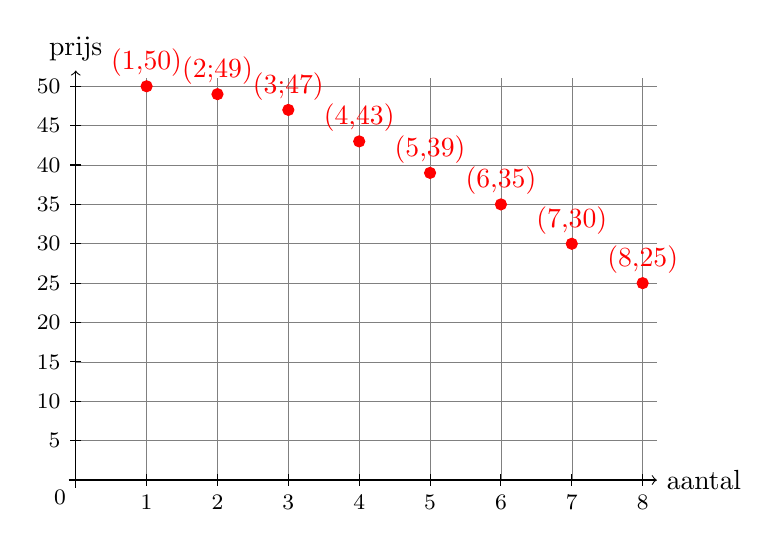
\begin{tikzpicture}[x=0.9cm,y=0.1cm]
\draw[help lines] (0,0) grid [xstep=1, ystep=5] (8.2,51);
\draw[->] (-0.1,0) -- (8.2,0) node[right] {aantal};
\draw[->] (0,-1) -- (0,52) node[above] {prijs};
\foreach \x in {1,...,8}
	\draw[shift={(\x,0)}] (0pt,2pt) -- (0pt,-2pt) node[below] {\footnotesize $\x$};
\foreach \y in {5,10,...,50}
	\draw[shift={(0,\y)},color=black] (2pt,0pt) -- (-2pt,0pt) node[left] {\footnotesize $\y$};
\node [below left] at (0,0) {\footnotesize 0};
\filldraw [red] (1,50) circle (2pt) node[above] {(1,50)};
\filldraw [red] (2,49) circle (2pt) node[above] {(2;49)};
\filldraw [red] (3,47) circle (2pt) node[above] {(3;47)};
\filldraw [red] (4,43) circle (2pt) node[above] {(4,43)};
\filldraw [red] (5,39) circle (2pt) node[above] {(5,39)};
\filldraw [red] (6,35) circle (2pt) node[above] {(6,35)};
\filldraw [red] (7,30) circle (2pt) node[above] {(7,30)};
\filldraw [red] (8,25) circle (2pt) node[above] {(8,25)};
\end{tikzpicture}
    \label{fig:grafieksportschoenen}
}\qquad
\subfloat[grafiek horende bij \cref{tab:reclame}]{
\begin{tikzpicture}[x=1cm,y=2cm]
%\draw[help lines] (0,0) grid [xstep=1, ystep=5] (8.5,3.5);
\draw[->] (-0.2,0) -- (8.2,0) node[right] {jaar na 2000};
\draw[->] (0,-0.2) -- (0,3.2) node[above] {Reclame-investeringen};
\foreach \x in {1,...,8}
	\draw[shift={(\x,0)}] (0pt,2pt) -- (0pt,-2pt) node[below] {\footnotesize $\x$};
\foreach \y in {0.5,1,...,3}
	\draw[shift={(0,\y)},color=black] (2pt,0pt) -- (-2pt,0pt) node[left] {\footnotesize $\y$};
\node [below left] at (0,0) {\footnotesize 0};
\filldraw [red] (1,1.752) circle (2pt);
\filldraw [red] (2,1.933) circle (2pt);
\filldraw [red] (3,2.137) circle (2pt) ;
\filldraw [red] (4,2.299) circle (2pt);
\filldraw [red] (5,2.387) circle (2pt);
\filldraw [red] (6,2.863) circle (2pt);
\filldraw [red] (7,3.089) circle (2pt);
\filldraw [red] (8,3.148) circle (2pt);
\end{tikzpicture}
    \label{fig:grafiekreclame}
}
\caption{Binaire relatie voorstellen in het twee-dimensionale vlak}
\end{figure}


\subsection{Functievoorschrift}\index{functievoorschift}
\label{subsec:voorschrift}
Bij een functievoorschrift noteer je op een eenduidige manier hoe de elementen van bron- en beeldverzameling met mekaar in verband staan. Dat is enkel mogelijk als dat verband onafhankelijk van de elementen van de bronverzameling  bepaald kan worden. Bij de kostprijs van de sportschoenen is dat bijvoorbeeld niet mogelijk.

Voorbeelden
\begin{itemize}
\item Bij een zwemmarathon sponsort de buurman je prestatie als volgt: \euros{6} startvergoeding en \euros{5} per kilometer (uitgedrukt als reëel getal).  Als je  $x$ \si{\kilo\meter} zwemt, betaalt de buurman  $y=6+5\cdot x$. Dit geeft de relatie
\[
U=\left\{(x,y)\mid x,y\in\real^+ \mathrm{~en~} y=6+5\cdot x\right\}
\]
\item Om op onze vakantiebestemming te geraken moeten we \SI{1323}{\km} afleggen. We rijden gemiddeld \SI{100}{\km\per\hour}. Als $t$ gelijk is aan de tijd  die we reeds in de auto doorbrachten uitgedrukt in uren, geeft volgende relatie  de resterende reistijd $r$ weer:
\[
V=\left \{(t,r)\mid t,r\in \real^+\mathrm{~en~} r=\frac{1323}{100}-t\right \}
\]
\end{itemize}


Het verband tussen de koppels $(x,y)$ van de relatie kan je schrijven als $y=f(x)$. In het voorgaande voorbeeld 
van de zwemmarathon is $f(x)=6+5\cdot x$.  Het getal $y$ noemen we de \emph{functiewaarde}\index{functiewaarde}. We noteren de relatie kort met $f$.  We schrijven ook
\[
f: \real\to\real: x\mapsto y =f(x)
\]
Deze notatie lezen we als `de relatie $f$ van $\real$ naar $\real$ waarbij $x$ wordt afgebeeld op $y$ en $y=f(x)$. Het spreekt voor zich dat je in plaats van de letter $f$ ook andere letters mag gebruiken, bijvoorbeeld $h$, $r$, \dots

Het functievoorschrift kan je ook gebruiken voor niet-binaire relaties. De relatie onderaan \cref{sec:defRelatie} kan je beschrijven met het voorschrift
\[
u:\real^2\to\real:(a,b)\mapsto c =a+b
\]

Het is heel belangrijk dat je bij deze notatie goed vermeldt wat het domein is van de functie. Zo heeft de relatie $\text{wortel}(x)=\sqrt{x}$ geen zin als de bronverzameling $\real$ is: je kan immers geen vierkantswortel berekenen van een negatief getal.

\subsection{Algoritme}\index{algoritme}
Als de functie voorgesteld wordt met een functievoorschrift, kan je het beeld  $y$ rechtstreeks berekenen uit $x$. Dat is niet altijd mogelijk: soms zijn er enkele `tussenstappen' nodig. Neem het volgende voorbeeld:
\begin{itemize}
\item Het is solden. Iedere klant krijgt 30\% korting. Als het totaal van de oorspronkelijke prijzen groter is dan \euros{100}, krijgt de klant 40\% korting. Als het totaal groter is dan \euros{200}, krijgt de klant 50\% korting. 
\end{itemize}
Als we een functie willen bepalen die het totaal $t$ van de oorspronkelijke prijzen afbeeldt op het te betalen bedrag $b$, moeten we in stappen werken:
\begin{enumerate}
\item Is $t<100$? Dan is $b=0,70\cdot t$
\item Is $100\leqslant t<200$? Dan is $b=0,60\cdot t$
\item Anders: $b=0,50\cdot t$
\end{enumerate}

Er is dus een werkwijze, een \emph{algoritme} nodig om de functie te bepalen. Dit brengt ons tot een verband tussen wiskunde en (functioneel) programmeren\footnote{Functioneel programmeren is niet hetzelfde als object-geori\"enteerd programmeren. Een methode op een object kan wel `functioneel' zijn. \url{http://nl.wikipedia.org/wiki/Functioneel_programmeren}}. Soms is het nodig om een programma te schrijven om een wiskundige functie te berekenen. In dit OPO gebruiken we Scilab als programmeertaal (zie \cref{scilab}). Bovenstaande functie kan in Scilab als volgt geprogrammeerd worden\footnote{Je kan ook een ‘elseif’ i.p.v. een ‘else if’ gebruiken, met een licht andere syntaxis.}:

\begin{verbatim}
function b=bedrag(t)
  if t<100 then
    b=0.70*t
  else 
    if t<200 then
      b=0.60*t
    else
      b=0.50*t
    end
  end
endfunction
\end{verbatim} 

Met de Scilab-functie \verb/plot/\index{plot} kan je de grafiek van de functie tekenen (zie \cref{fig:solden}).
Uit deze grafiek blijkt dat je vriendin beter nog een T-shirt extra koopt als ze al een bedrag van \euros{85} besteed heeft.

\begin{figure}[htpb]
\centering
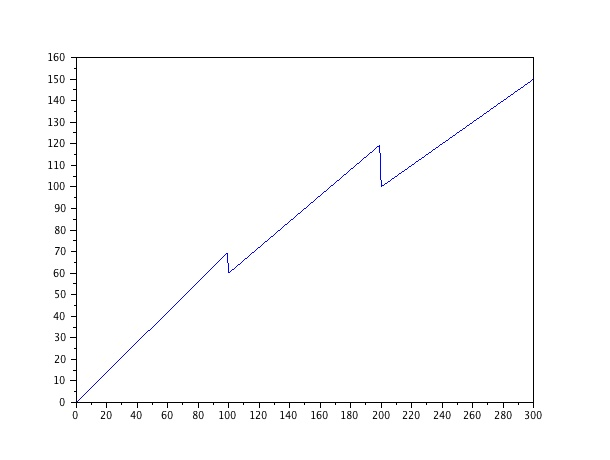
\includegraphics[width=0.7\textwidth]{figuren/verzamelingen_relaties/solden.jpeg}
\caption{Grafiek van de functie \texttt{bedrag}, getekend in Scilab.}
\label{fig:solden}
\end{figure}

Een algoritme kan ook \emph{recursief}\index{recursief}\index{algoritme!recursief} zijn: uit de functiewaarde van het ene element leid je de functiewaarde van een ander element af. Voorbeeld hiervan is de functie die de waarde van $n!$ berekent. Immers $n!=n\cdot(n-1)!$. We verwijzen naar de OPO's `Algoritmen en datastructuren' voor meer details.



We vermelden ten slotte dat binaire relaties ook voorgesteld kunnen worden met grafen\footnote{\url{http://nl.wikipedia.org/wiki/Grafen}} en matrices\footnote{\url{http://nl.wikipedia.org/wiki/Matrix_(wiskunde)}}. Deze leerstof wordt behandeld in het OPO `Toegepaste Wiskunde 2'.

\section{Inverse relatie}\index{inverse relatie}\index{relatie!inverse}
\label{sec:invrelatie}
Een relatie kan je `inverteren: je verwisselt bron en beeld met mekaar.
\begin{quote}
Zij $U$ een relatie van $A$ naar $B$: 
\[U=\{({x},{y})\mid {x}\in A \mathrm{~en~}{y}\in B\},\]
dan is de inverse relatie van $U$ gelijk aan 
\[U^{-1}=\{({y},{x})\mid ({x},{y})\in U \}\]
\end{quote}
Het komt erop neer dat je in de koppels $({x},{y})$ de $x$ en $y$ van plaats wisselt.


Is de inverse van een functie altijd opnieuw een functie?  In \cref{subsec:functies} gaven we aan dat een relatie een functie is waarbij elke $x$ hoogstens één beeld heeft. Neem de functie $f:\real\to\real:x\mapsto y= x^2$. Het getal \num{4} is beeld van zowel $x=2$ als $x=-2$. Voor de inverse functie moet je $x$ en $y$ met mekaar verwisselen, maar neem je dan 2 als invers beeld voor 4 of $-2$? We besluiten hieruit dat de inverse relatie van een functie niet altijd een functie is. Als de functie \emph{injectief} is, is de inverse van die functie wél een functie. 

Voorbeelden
\begin{itemize}
\item als $U$ de relatie `student $x$ heeft inschrijvingsnummer $y$', dan is de inverse relatie $U^{-1}$ de relatie `inschrijvingsnummer $y$ hoort bij student $x$'
\item als $V$ de relatie 'computer met serienummer $x$ is eigendom van persoon $y$', dan is de inverse relatie $V^{-1}$ de relatie 'persoon $y$ is eigenaar van computer met serienummer $x$'
\item gegeven de relatie $W=\{(x,y)\mid x,y\in \integers \mathrm{~en~} y=x+3\}$ dan is $W^{-1}=\{(a,b)\mid a,b\in \integers \mathrm{~en~} b=a-3\}$.
\end{itemize}




Als laatste bespreken we de inverse van een functie die omschreven wordt door een functievoorschrift. 
Neem het voorbeeld van de functie $f(x)=6+5\cdot x$ uit \cref{subsec:voorschrift} die het aantal gezwommen kilometers afbeeldt op het te betalen bedrag. De grafiek van deze functie wordt ook getoond in \cref{fig:fotos}. Op deze grafiek zie je duidelijk dat bij elke $x$ juist \'e\'en $y$ hoort. De functie is dus \'e\'en-op-\'e\'en en kan dus ge\"inverteerd worden. We moeten  de waarde van $x$ zoeken als we $y$ kennen. Als $y=20$, kunnen we op de grafiek aflezen dat $x\approx \num{2.8}$. Als je bij buurman \euros{20} sponsorgeld wil verdienen, moet je ongeveer \SI{2.8}{\kilo\meter} zwemmen. 

\begin{figure}[htbp]
\centering
\begin{tikzpicture}[x=2cm,y=0.25cm]
\draw[->] (-0.2,0) -- (5.2,0) node[right] {$x$};
\draw[->] (0,-1) -- (0,32) node[above] {$f(x)$};
\foreach \x in {0.5,1,...,5}
	\draw[shift={(\x,0)}] (0pt,2pt) -- (0pt,-2pt) node[below] {\footnotesize $\x$};
\foreach \y in {5,10,...,30}
	\draw[shift={(0,\y)},color=black] (2pt,0pt) -- (-2pt,0pt) node[left] {\footnotesize $\y$};
\draw[thick](0,6) -- (5,31);
\node [below left] at (0,0) {\footnotesize 0};
\draw[dashed,-latex](0,20) -- (2.8,20);
\draw[dashed, -latex](2.8,20) -- (2.8,0);
\filldraw [red] (2.8,20) circle (2pt);
\end{tikzpicture}
\caption{Grafiek van de functie $f(x)=6+5\cdot x$ }
\label{fig:fotos}
\end{figure}

Wil je exact weten hoeveel kilometer je moet zwemmen om \euros{20} te krijgen van buurman, kan je het functievoorschrift gebruiken:
\[
\begin{split}
y&=6+5\cdot x\\
& \Updownarrow\\
x&=\frac{y-6}{5}
\end{split}
\]
Als buurman \euros{20} betaalt, heb je $x=\frac{20-6}{5}=\frac{14}{5}=2,8$ kilometer gezwommen.

\section{Samenvatting}
\begin{description}
  \item[relatie] Een \emph{relatie} over verzamelingen $A_1, A_2, \dots, A_n$ is een deelverzameling van $A_1 \times A_2 \times \dots \times A_n$.
  \item[binaire relatie] Een \emph{binaire relatie} met \emph{bronverzameling} $A$ en \emph{doelverzameling} $B$ is een deelverzameling van $A \times B$.
    \[ R \subset A \times B \]
  \item[domein] Het \emph{domein} van een binaire relatie $R$ is
    \[ \dom{R} = \{ \; x \;|\; \exists y. \; (x, y) \in R \; \} \]
  \item[bereik] Het \emph{bereik} van een binaire relatie $R$ is
    \[ \range{R} = \{ \; y \;|\; \exists x. \; (x, y) \in R \; \} \]
  \item[functie] Een \emph{functie} $R \subset A \times B$ is een binaire relatie waarvoor geldt er voor elke $x \in A$ maximaal \'e\'en $y \in B$ bestaat waarvoor geldt dat $(x,y) \in R$.
  \item[afbeelding] Een \emph{afbeelding} $R \subset A \times B$ is een functie waarvoor geldt er voor elke $x \in A$ exact \'e\'en $y \in B$ bestaat waarvoor geldt dat $(x, y) \in R$.
  \item[surjectie] Een \emph{surjectie} $R \subset A \times B$ is een functie waarvoor geldt dat voor elke $y \in B$ er een $x \in A$ bestaat zodat $(x, y) \in R$.
  \item[injectie] Een \emph{injectie} $R \subset A \times B$ is een functie waarvoor geldt dat voor elke $y \in B$ er een unieke $x \in A$ bestaat zodat $(x, y) \in R$.
  \item[bijectie] Een \emph{bijectie} $R$ is een functie die zowel surjectief als injectief is.
  \item[inverse relatie] De \emph{inverse} van $R \subset A \times B$ is de relatie $R^{-1} \subset B \times A$ waarbij
    \[ R^{-1} = \{ \; (y, x) \;|\; (x, y) \in R \; \} \]
\end{description}

\section{Oefeningen}
\begin{oef}
\label{oef21}
$A = \{1, 3, 5, 7\}$ en  $B = \{2, 4, 6,8\}$. Noteer volgende relaties door middel van opsomming:
\begin{enumerate}
\item $U=\{(x,y) \mid x\in A \mathrm{~en~} y \in B \mathrm{~en~} x+y<9\}$
\item $V=\{(x,y) \mid x\in A \mathrm{~en~} y \in B  \mathrm{~en~} x<y \}$
\end{enumerate}
\begin{opl}
\begin{enumerate}
\item $U=\{(1,2),(1,4),(1,6),(3,2),(3,4),(5,2) \}$
\item $V=\{(1,2),(1,4),(1,6),(1,8),(3,4),(3,6),(3,8),(5,6),(5,8),(7,8) \}$
\end{enumerate}
\end{opl}
\end{oef}

\begin{oef}
\begin{enumerate}
\item Bepaal domein en bereik van de relaties van oefening~2.1.
\item Geef de meest correcte benaming van de relaties.
\end{enumerate}
\begin{opl}
\begin{enumerate}
\item $\dom{U}=\{1,3,5 \}$; $\range{U}=\{2,4,6 \}$; relatie, geen injectie (want bvb. in het element 2 komen drie pijlen toe) of surjectie (want in het element 8 komt geen pijl toe). De relatie is geen functie want er zijn elementen met meer dan \'e\'en beeld (bvb. het element 1 heeft drie beelden).
\item $\dom{V}=\{1,3,5,7 \}$; $\range{V}=\{2,4,6,8 \}$; surjectieve relatie
\end{enumerate}
\end{opl}
\end{oef}




\begin{oef}
Gegeven $X = \{\mathrm{a},\mathrm{ b}\}$ en $Y = \{\mathrm{c}, \mathrm{d}, \mathrm{e}, \mathrm{f}\}$. Noteer volgende productverzamelingen door middel van opsomming:
\begin{enumerate}
\item $X\times Y$
\item $Y\times X$
\item $X^2$
\end{enumerate}
\begin{opl}
\begin{enumerate}
\item $X\times Y=\{(a,c),(a,d),(a,e),(a,f),(b,c),(b,d),(b,e),(b,f) \}$
\item $Y\times X=\{(c,a),(c,b),(d,a),(d,b),(e,a),(e,b),(f,a),(f,b) \}$
\item $X^2=\{(a,a),(a,b),(b,a),(b,b) \}$
\end{enumerate}
\end{opl}
\end{oef}

\begin{oef}
Een e-mailadres kan je beschouwen als  een productverzameling van drie verzamelingen. Noteer deze verzamelingen zorgvuldig en definieer de gevraagde productverzameling.
\begin{opl}
$A=\{\text{strings bestaande uit a-zA-Z,.,0-9} \}$\\
$B=\{\text{strings bestaande uit a-zA-Z,.} \}$\\
$C=\{ \text{strings uit de lijst met goedgekeurde TLD's (Top Level Domain names}\}$\\
$A\times B\times C$
\end{opl}
\end{oef}

\begin{oef}
Hieronder vind je een aantal relaties van verzameling $A$ naar $B$. 
\begin{itemize}
\item Definieer voor elk van de gevallen de verzamelingen $A$ en $B$ eenduidig. Er zijn verschillende mogelijkheden.
\item Zoek een gepaste voorstellingswijze voor de relatie
\item Bepaal  welk soort relatie er beschreven wordt.
\end{itemize}
\begin{enumerate}
\item Klant heeft contactmoment
\item Klant heeft id
\item Persoon woont op adres
\item Student heeft telefoonnummer
\item Student krijgt rapport
\item Student volgt OPO
\end{enumerate}
\begin{opl}
\begin{enumerate}

\item Klant heeft contactmoment: $A$=$\{\text{klanten van het bedrijf}\}$; \\
$B=\{\text{mogelijke contactmomenten voor manager}\}$; 
\'e\'en klant kan meerdere contactmomenten hebben, maar is er niet toe verplicht; 
niet alle mogelijke contactmomenten moeten ingevuld worden, maar nooit meer dan \'e\'en klant per contactmoment: injectieve relatie

\item Klant heeft id: $A$=$\{\text{klanten van het bedrijf}\}$; \\
$B=\{\text{id's die de software toegekend heeft}\}$ 
iedere klant heeft juist \'e\'en id: bijectie (afbeelding die bijectief is)

\item Persoon woont op adres: $A=\{\text{mensen met een geregistreerd adres}\}$; \\
$B=\{\text{geregistreerde adressen}\}$; iedere persoon woont op \'e\'en adres; op \'e\'en adres kunnen meerdere personen wonen: surjectie (afbeelding die surjectief is); als $A$ ook daklozen bevat: surjectieve functie

\item Student heeft telefoonnummer: $A=\{\text{studenten KHLeuven}\}$; \\
$B=\{$telefoonnummers die in het studentenregistratiesysteem opgenomen zijn$\}$.  Iedere student heeft nul, \'e\'en of meerdere telefoonnummers; ieder telefoonnummer heeft \'e\'en eigenaar: bijectieve relatie.
Als je broers en zussen toelaat als student: surjectieve relatie want telefoonnummer kan horen bij verschillende studenten.

\item Student krijgt rapport: $A=\{\text{leerlingen van KHLeuven}\}$; \\
$B=\{\text{afgedrukte rapporten op het einde van een examenperiode}\}$ voor elke student is er juist \'e\'en rapport: bijectie (afbeelding die bijectief is)

\item Student volgt OPO: $A=\{\text{studenten van KHLeuven}\}$; \\
$B=\{\text{OPO's die de KHLeuven inricht}\}$ student volgt meerdere OPO's en elk OPO wordt door meerdere studenten gevolgd: surjectieve relatie, tenzij er OPO's zijn die door geen enkele student gevolgd worden (dat zou kunnen gebeuren bij keuzeOPO's bvb). In dat geval is het een gewone relatie.
\end{enumerate}

\end{opl}
\end{oef}

\begin{oef}\label{oef:26}
Definieer volgende relaties correct:
\begin{itemize}
  \item Bepaal bron- en doelverzameling zodat de relatie een bijectie is.
  \item Stel de relatie voor als een verzameling van paren door middel van een functievoorschrift, bijv.\ $U=\{(x,y)|x,y\in \real\text{ en } y=x+1\}$
  \item Geef nog minstens \'e\'en andere voorstellingswijze
\end{itemize}
\begin{enumerate}
  \item de functie $y=\sqrt{x}$
  \item de relatie die de kostprijs van de brandstof van een autorit weergeeft
        in functie van de lengte van de rit (uitgedrukt in kilometers). De auto
        verbruikt \SI{6,45}{\litre} per \SI{100}{\kilo\meter}. De brandstof kost \euros{1,315} per liter.
  \item de relatie die de prijs van de factuur van een mazoutlevering weergeeft
        in functie van het aantal gekochte liter. Mazout kost \euros{0,9155} per
        liter als je minder dan \SI{2000}{\litre} afneemt en \euros{0,8887}
        per liter als je meer dan \SI{2000}{\litre} afneemt.
\end{enumerate}
\begin{opl}
\begin{enumerate}
  \item \begin{enumerate}
          \item bron- en beeldverzameling: $\real^+$
          \item $U=\{(x,y)|x,y\in \real^+\text{ en } y=\sqrt{x} \}$
          \item zie figuur~\ref{oef:opl26}
                \begin{figure}[htbp]
                  \centering
                  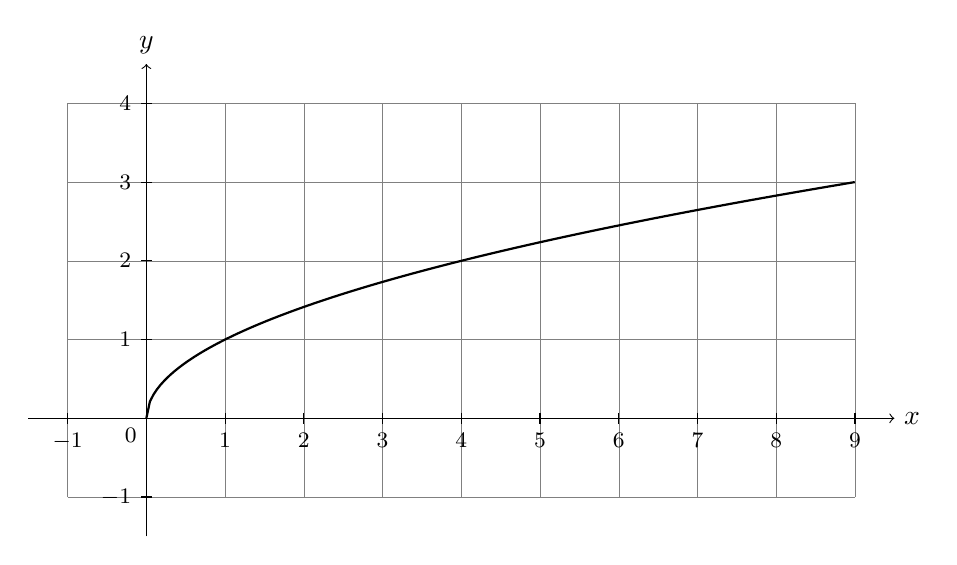
\begin{tikzpicture}[x=1cm,y=1cm]
                  \draw[help lines] (-1,-1) grid (9,4);
                  \draw[->] (-1.5,0) -- (9.5,0) node[right] {$x$};
                  \draw[->] (0,-1.5) -- (0,4.5) node[above] {$y$};
                  \foreach \x in {-1,1,2,...,9}
                          \draw[shift={(\x,0)}] (0pt,2pt) -- (0pt,-2pt) node[below] {\footnotesize $\x$};
                  \foreach \y in {-1,1,2,...,4}
                          \draw[shift={(0,\y)},color=black] (2pt,0pt) -- (-2pt,0pt) node[left] {\footnotesize $\y$};
                  \draw [domain=0:9,samples=200,thick] plot(\x,{sqrt(\x)});
                  \node [below left] at (0,0) {\footnotesize 0};
                  \end{tikzpicture}
                  \caption{Oplossing van oefening~\ref{oef:26}}\label{oef:opl26}
                \end{figure}
        \end{enumerate}
  \item \begin{enumerate}
          \item bron- en beeldverzameling is  $\real^+$
          \item $U=\{(x,y)|x,y\in \real^+\text{ en } y=8,48175\cdot x/100\}$
        \end{enumerate}
  \item \begin{enumerate}
          \item bron- en beeldverzameling is  $\real^+$
          \item $U = \left\lbrace (x,y)\;|\; x,y \in \real^+
                \text{ en } y = \begin{cases}
                                  0,9155\cdot x&\text{ als }x<2000\\
                                  0,8887\cdot x&\text{ anders }
                                \end{cases} \qquad \right\rbrace$
        \end{enumerate}

\end{enumerate}
\end{opl}
\end{oef}

\begin{oef}
Wat is de inverse van volgende relaties? Stel de relatie voor op dezelfde manier als de opgave.
\begin{enumerate}
  \item $\{(1,7),(2,10),(3,9) \}$
  \item \begin{tabular}{c|cccccc}
          $x$ & \num{0.1} & \num{0.2} & \num{0.3} & \num{0.4} & \num{0.5} & \num{0.6} \\ 
          \midrule
          $y$ & 2 & 4 & 6 & 8 & 10 & 12 \\ 
        \end{tabular} 
  \item $f: \real\rightarrow\real:x\mapsto y \mid y=2\cdot x+10 $
  \item $f: \real^+\rightarrow\real:x\mapsto y \mid y=\sqrt{x}$
\end{enumerate}
\begin{opl}
\begin{enumerate}
  \item \{(7,1),(10,2),(9,3) \}
  \item \begin{tabular}{c|cccccc}
          $y$ & 2 & 4 & 6 & 8 & 10 & 12 \\ 
          \midrule
          $x$ & \num{0.1} & \num{0.2} & \num{0.3} & \num{0.4} & \num{0.5} & \num{0.6} \\ 
        \end{tabular} 
  \item $f^{-1}: \real\rightarrow\real:x\mapsto  y=\dfrac{x-10}{2} $
  \item $f^{-1}: \real^+\rightarrow\real^+:x\mapsto y=x^2$
\end{enumerate}
\end{opl}
\end{oef}



\begin{oef}
Zelfde vraag voor elke figuur:
\begin{itemize}
  \item Teken de inverse functie.
  \item Wat is het functievoorschrift van de getekende functie en zijn inverse?
\end{itemize}
\begin{enumerate}
  \begin{minipage}{\columnwidth}
    \item 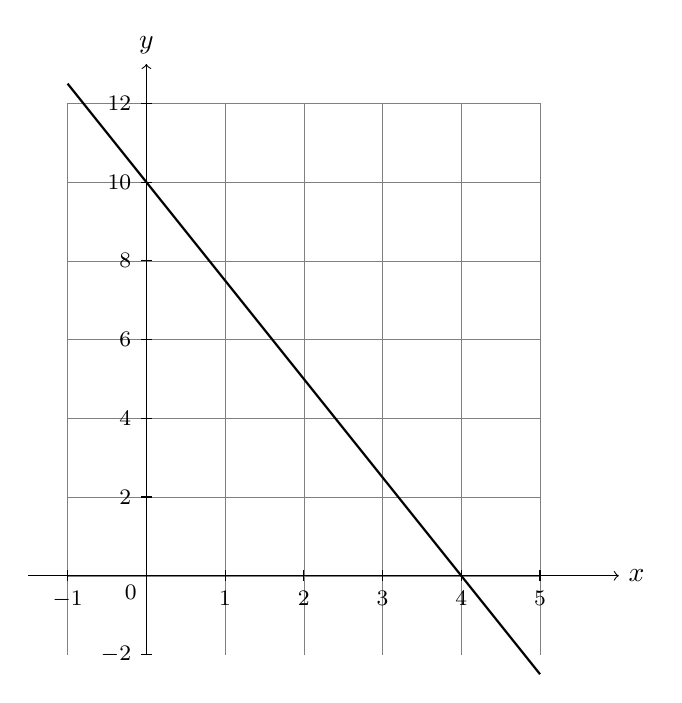
\begin{tikzpicture}[x=1cm,y=.5cm]
            \draw[help lines] (-1,-2) grid (5,12);
            \draw[->] (-1.5,0) -- (6,0) node[right] {$x$};
            \draw[->] (0,-2) -- (0,13) node[above] {$y$};
            \foreach \x in {-1,1,2,...,5}
                    \draw[shift={(\x,0)}] (0pt,2pt) -- (0pt,-2pt) node[below] {\footnotesize $\x$};
            \foreach \y in {-2,2,4,...,12}
                    \draw[shift={(0,\y)},color=black] (2pt,0pt) -- (-2pt,0pt) node[left] {\footnotesize $\y$};
            \draw[thick](5,-2.5) -- (-1,12.5); % rechte 1
            \node [below left] at (0,0) {\footnotesize 0};
          \end{tikzpicture}
  \end{minipage}
  \begin{minipage}{\columnwidth}
    \item 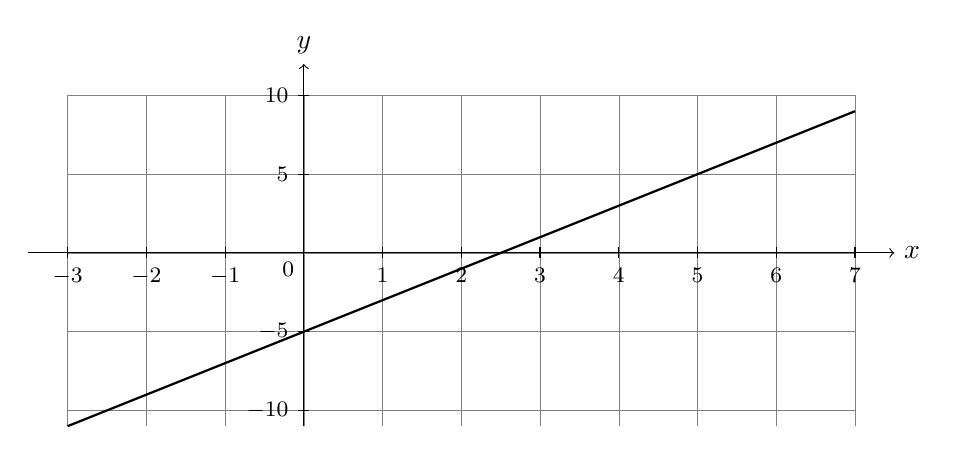
\begin{tikzpicture}[x=1cm,y=.2cm]
            \draw[help lines] (-3,-11) grid (7,10);
            \draw[->] (-3.5,0) -- (7.5,0) node[right] {$x$};
            \draw[->] (0,-11) -- (0,12) node[above] {$y$};
            \foreach \x in {-3,-2,-1,1,2,...,7}
                    \draw[shift={(\x,0)}] (0pt,2pt) -- (0pt,-2pt) node[below] {\footnotesize $\x$};
            \foreach \y in {-10,-5,5,10}
                    \draw[shift={(0,\y)},color=black] (2pt,0pt) -- (-2pt,0pt) node[left] {\footnotesize $\y$};
            \draw[thick](-3,-11) -- (7,9); % rechte 1
            \node [below left] at (0,0) {\footnotesize 0};
          \end{tikzpicture}
  \end{minipage}
  \begin{minipage}{\columnwidth}
    \item 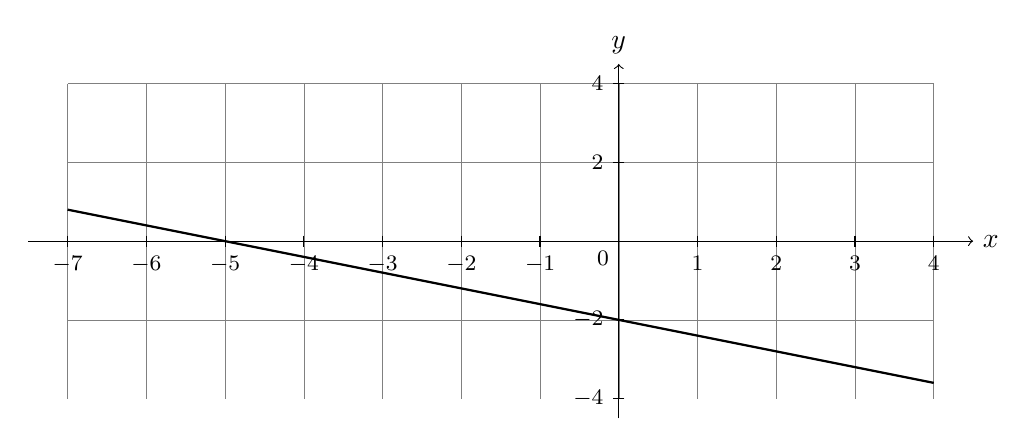
\begin{tikzpicture}[x=1cm,y=.5cm]
            \draw[help lines] (-7,-4) grid (4,4);
            \draw[->] (-7.5,0) -- (4.5,0) node[right] {$x$};
            \draw[->] (0,-4.5) -- (0,4.5) node[above] {$y$};
            \foreach \x in {-7,-6,...,-1,1,2,...,4}
                    \draw[shift={(\x,0)}] (0pt,2pt) -- (0pt,-2pt) node[below] {\footnotesize $\x$};
            \foreach \y in {-4,-2,2,4}
                    \draw[shift={(0,\y)},color=black] (2pt,0pt) -- (-2pt,0pt) node[left] {\footnotesize $\y$};
            \draw[thick](-7,0.8) -- (4,-3.6); % rechte 1
            \node [below left] at (0,0) {\footnotesize 0};
          \end{tikzpicture}
  \end{minipage}
\end{enumerate}

\begin{opl}
\begin{enumerate}
\item $y=-\frac52 x +10$; inverse functie: $y=-\frac25 x +4$
\item $y=2x-5$; inverse functie: $y=\frac12 x+\frac52$
\item $y=-\frac25x-2$; inverse functie: $y=-\frac52x-5$
\end{enumerate}
\end{opl}
\end{oef}



\begin{oef}
De volgende grafieken stellen relaties voor met als bronverzameling $A$ en doelverzameling $B$ het interval $[0,1]$. Geef voor elk van de relaties aan of deze
functies, afbeeldingen, injectief, surjectief en/of bijectief zijn.
\begin{center}
  \newcommand{\axes}{
    \path[use as bounding box] (-.5,-.5) rectangle (4,4);
    \draw[step=3cm,gray,thin] (-.5,-.5) grid (4,4);
    \draw[thin,->] (-.5,0) -- (4,0) node[at end,above left] {$A$};
    \draw[thin,->] (0,-.5) -- (0,4) node[at end,left] {$B$};
  }
  \begin{tabular}{cc}
    1.
    \begin{tikzpicture}
      \axes
      \draw[thick] (0,0) -- (1,1);
      \draw[thick] (2,2) -- (3,3);
    \end{tikzpicture}
    &
    2.
    \begin{tikzpicture}
      \axes
      \draw[thick] (0,0) to[out=90,in=-90] (3,3);
    \end{tikzpicture}
    \\
    3.
    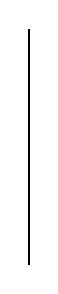
\begin{tikzpicture}
      \axes
      \draw[thick] (1.5,0) -- (1.5,3);
    \end{tikzpicture}
    &
    4.
    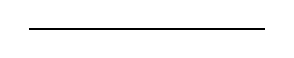
\begin{tikzpicture}
      \axes
      \draw[thick] (0,1.5) -- (3,1.5);
    \end{tikzpicture}
    \\
    5.
    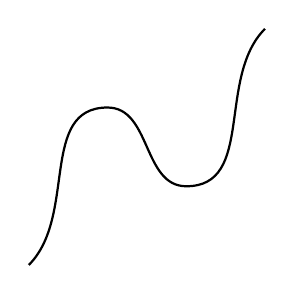
\begin{tikzpicture}
      \axes
      \draw[thick] (0,0) to[out=45,in=180] (1,2) to[out=0,in=180] (2,1) to[out=0,in=225] (3,3);
    \end{tikzpicture}
    &
    6.
    
\begin{tikzpicture}
      \axes
      \draw[thick] (1.5,1.5) circle (1cm);
    \end{tikzpicture}
  \end{tabular}
\end{center}
\begin{opl}
  \hspace{1mm}
  \begin{center}
    \begin{tabular}{cccccc}
      & \rotatebox{90}{functie}
      & \rotatebox{90}{afbeelding}
      & \rotatebox{90}{injectief}
      & \rotatebox{90}{surjectief}
      & \rotatebox{90}{bijectief} \\
      \toprule
      1. & \checkmark &            & \checkmark &            & \checkmark \\
      2. & \checkmark & \checkmark & \checkmark & \checkmark & \checkmark \\
      3. &            &            &            & \checkmark &            \\
      4. & \checkmark & \checkmark &            &            &            \\
      5. & \checkmark & \checkmark &            & \checkmark &            \\
      6. &            &            &            &            &            \\
    \end{tabular}
  \end{center}
\end{opl}
\end{oef}

%%% Local Variables: 
%%% mode: latex
%%% TeX-master: "../cursusTW1"
%%% End: 


%%% Local Variables: 
%%% mode: latex
%%% TeX-master: "cursusTW1"
%%% End: 
